\begin{verbatim}
    Sondagem Linear (7 colisões):
\end{verbatim}

% Insert 10
\begin{center}
    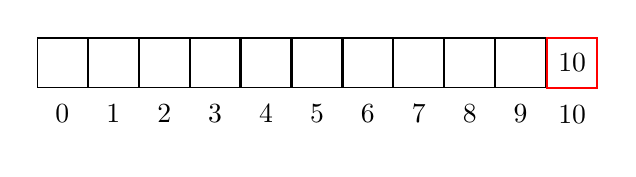
\begin{tikzpicture}
        \tikzstyle{every node}=[draw, minimum size=1.8em]
        
        \matrix[draw=none] {
            \node   (0)    [label=270:$0$] {}; & 
            \node   (1)    [label=270:$1$] {}; &
            \node   (2)    [label=270:$2$] {}; & 
            \node   (3)    [label=270:$3$] {}; &
            \node   (4)    [label=270:$4$] {}; & 
            \node   (5)    [label=270:$5$] {}; &
            \node   (6)    [label=270:$6$] {}; &
            \node   (7)    [label=270:$7$] {}; &
            \node   (8)    [label=270:$8$] {}; &
            \node   (9)    [label=270:$9$] {}; &
            \node   (10)   [label=270:$10$, draw=red, thick] {10}; \\
        };
        
    \end{tikzpicture}
\end{center}

% Insert 22
\begin{center}
    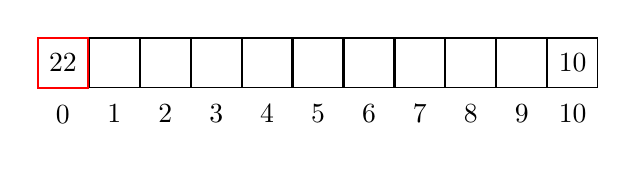
\begin{tikzpicture}
        \tikzstyle{every node}=[draw, minimum size=1.8em]
        
        \matrix[draw=none] {
            \node   (0)    [label=270:$0$, draw=red, thick] {22}; & 
            \node   (1)    [label=270:$1$] {}; &
            \node   (2)    [label=270:$2$] {}; & 
            \node   (3)    [label=270:$3$] {}; &
            \node   (4)    [label=270:$4$] {}; & 
            \node   (5)    [label=270:$5$] {}; &
            \node   (6)    [label=270:$6$] {}; &
            \node   (7)    [label=270:$7$] {}; &
            \node   (8)    [label=270:$8$] {}; &
            \node   (9)    [label=270:$9$] {}; &
            \node   (10)   [label=270:$10$] {10}; \\
        };
        
    \end{tikzpicture}
\end{center}

% Insert 31
\begin{center}
    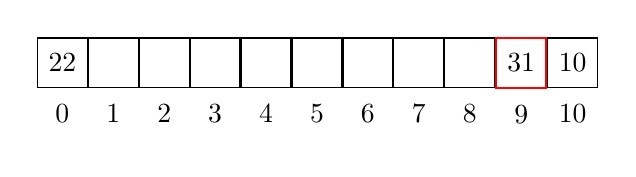
\begin{tikzpicture}
        \tikzstyle{every node}=[draw, minimum size=1.8em]
        
        \matrix[draw=none] {
            \node   (0)    [label=270:$0$] {22}; & 
            \node   (1)    [label=270:$1$] {}; &
            \node   (2)    [label=270:$2$] {}; & 
            \node   (3)    [label=270:$3$] {}; &
            \node   (4)    [label=270:$4$] {}; & 
            \node   (5)    [label=270:$5$] {}; &
            \node   (6)    [label=270:$6$] {}; &
            \node   (7)    [label=270:$7$] {}; &
            \node   (8)    [label=270:$8$] {}; &
            \node   (9)    [label=270:$9$, draw=red, thick] {31}; &
            \node   (10)   [label=270:$10$] {10}; \\
        };
        
    \end{tikzpicture}
\end{center}

% Insert 4
\begin{center}
    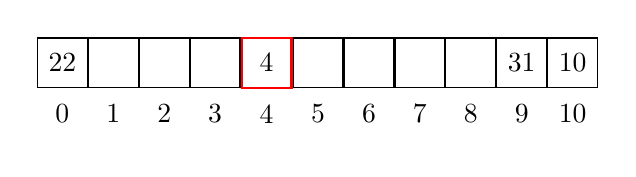
\begin{tikzpicture}
        \tikzstyle{every node}=[draw, minimum size=1.8em]
        
        \matrix[draw=none] {
            \node   (0)    [label=270:$0$] {22}; & 
            \node   (1)    [label=270:$1$] {}; &
            \node   (2)    [label=270:$2$] {}; & 
            \node   (3)    [label=270:$3$] {}; &
            \node   (4)    [label=270:$4$, draw=red, thick] {4}; & 
            \node   (5)    [label=270:$5$] {}; &
            \node   (6)    [label=270:$6$] {}; &
            \node   (7)    [label=270:$7$] {}; &
            \node   (8)    [label=270:$8$] {}; &
            \node   (9)    [label=270:$9$] {31}; &
            \node   (10)   [label=270:$10$] {10}; \\
        };
        
    \end{tikzpicture}
\end{center}

% Insert 15
\begin{center}
    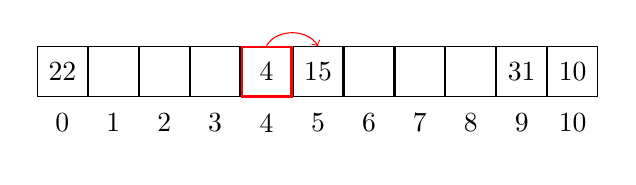
\begin{tikzpicture}
        \tikzstyle{every node}=[draw, minimum size=1.8em]
        
        \matrix[draw=none] {
            \node   (0)    [label=270:$0$] {22}; & 
            \node   (1)    [label=270:$1$] {}; &
            \node   (2)    [label=270:$2$] {}; & 
            \node   (3)    [label=270:$3$] {}; &
            \node   (4)    [label=270:$4$, draw=red, thick] {4}; & 
            \node   (5)    [label=270:$5$] {15}; &
            \node   (6)    [label=270:$6$] {}; &
            \node   (7)    [label=270:$7$] {}; &
            \node   (8)    [label=270:$8$] {}; &
            \node   (9)    [label=270:$9$] {31}; &
            \node   (10)   [label=270:$10$] {10}; \\
        };
        
        \draw[->, red, out=60, in=120] (4.north) to (5.north);
        
    \end{tikzpicture}
\end{center}

% Insert 28
\begin{center}
    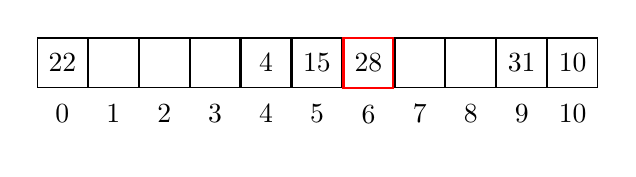
\begin{tikzpicture}
        \tikzstyle{every node}=[draw, minimum size=1.8em]
        
        \matrix[draw=none] {
            \node   (0)    [label=270:$0$] {22}; & 
            \node   (1)    [label=270:$1$] {}; &
            \node   (2)    [label=270:$2$] {}; & 
            \node   (3)    [label=270:$3$] {}; &
            \node   (4)    [label=270:$4$] {4}; & 
            \node   (5)    [label=270:$5$] {15}; &
            \node   (6)    [label=270:$6$, draw=red, thick] {28}; &
            \node   (7)    [label=270:$7$] {}; &
            \node   (8)    [label=270:$8$] {}; &
            \node   (9)    [label=270:$9$] {31}; &
            \node   (10)   [label=270:$10$] {10}; \\
        };
        
    \end{tikzpicture}
\end{center}

% Insert 17
\begin{center}
    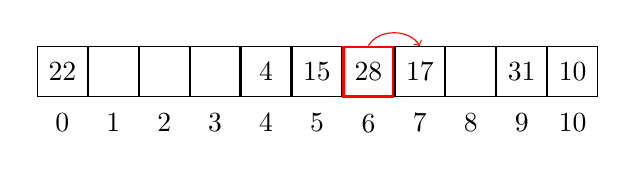
\begin{tikzpicture}
        \tikzstyle{every node}=[draw, minimum size=1.8em]
        
        \matrix[draw=none] {
            \node   (0)    [label=270:$0$] {22}; & 
            \node   (1)    [label=270:$1$] {}; &
            \node   (2)    [label=270:$2$] {}; & 
            \node   (3)    [label=270:$3$] {}; &
            \node   (4)    [label=270:$4$] {4}; & 
            \node   (5)    [label=270:$5$] {15}; &
            \node   (6)    [label=270:$6$, draw=red, thick] {28}; &
            \node   (7)    [label=270:$7$] {17}; &
            \node   (8)    [label=270:$8$] {}; &
            \node   (9)    [label=270:$9$] {31}; &
            \node   (10)   [label=270:$10$] {10}; \\
        };
        
        \draw[->, red, out=60, in=120] (6.north) to (7.north);
        
    \end{tikzpicture}
\end{center}

% Insert 88
\begin{center}
    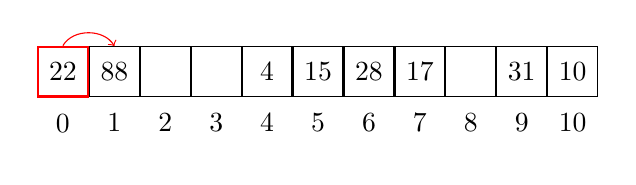
\begin{tikzpicture}
        \tikzstyle{every node}=[draw, minimum size=1.8em]
        
        \matrix[draw=none] {
            \node   (0)    [label=270:$0$, draw=red, thick] {22}; & 
            \node   (1)    [label=270:$1$] {88}; &
            \node   (2)    [label=270:$2$] {}; & 
            \node   (3)    [label=270:$3$] {}; &
            \node   (4)    [label=270:$4$] {4}; & 
            \node   (5)    [label=270:$5$] {15}; &
            \node   (6)    [label=270:$6$] {28}; &
            \node   (7)    [label=270:$7$] {17}; &
            \node   (8)    [label=270:$8$] {}; &
            \node   (9)    [label=270:$9$] {31}; &
            \node   (10)   [label=270:$10$] {10}; \\
        };
        
        \draw[->, red, out=60, in=120] (0.north) to (1.north);
        
    \end{tikzpicture}
\end{center}

% Insert 59
\begin{center}
    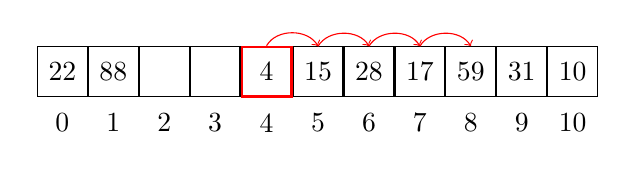
\begin{tikzpicture}
        \tikzstyle{every node}=[draw, minimum size=1.8em]
        
        \matrix[draw=none] {
            \node   (0)    [label=270:$0$] {22}; & 
            \node   (1)    [label=270:$1$] {88}; &
            \node   (2)    [label=270:$2$] {}; & 
            \node   (3)    [label=270:$3$] {}; &
            \node   (4)    [label=270:$4$, draw=red, thick] {4}; & 
            \node   (5)    [label=270:$5$] {15}; &
            \node   (6)    [label=270:$6$] {28}; &
            \node   (7)    [label=270:$7$] {17}; &
            \node   (8)    [label=270:$8$] {59}; &
            \node   (9)    [label=270:$9$] {31}; &
            \node   (10)   [label=270:$10$] {10}; \\
        };
    
        \path[->, red]  (4.north) edge [out=60, in=120] (5.north)
                        (5.north) edge [out=60, in=120] (6.north)
                        (6.north) edge [out=60, in=120] (7.north)
                        (7.north) edge [out=60, in=120] (8.north);
        
    \end{tikzpicture}
\end{center}